\documentclass[border=10pt]{standalone}
\usepackage{pgfplots}
\usepgfplotslibrary{colormaps}
\pgfplotsset{compat=1.18}

\begin{document}
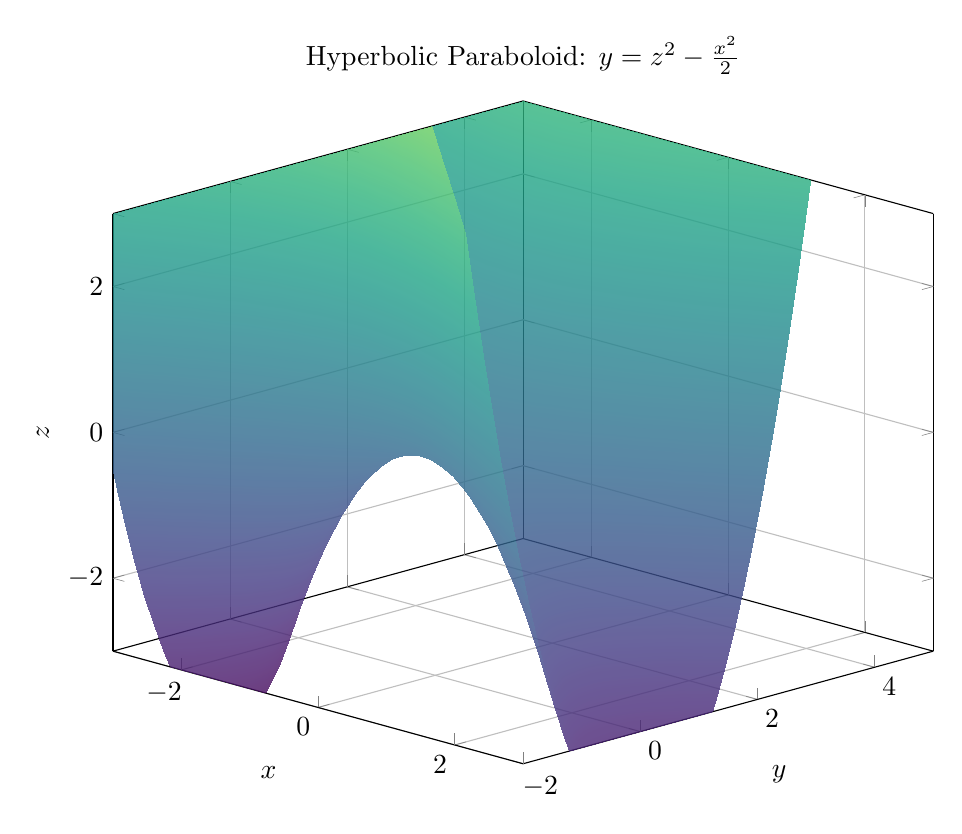
\begin{tikzpicture}
\begin{axis}[
    xlabel=$x$,
    ylabel=$y$,
    zlabel=$z$,
    title={Hyperbolic Paraboloid: $y = z^2 - \frac{x^2}{2}$},
    view={45}{20},
    colormap/viridis,
    width=12cm,
    height=10cm,
    grid=major,
    zmin=-3, zmax=3,
    xmin=-3, xmax=3,
    ymin=-2, ymax=5,
]
\addplot3[
    surf,
    shader=interp,
    domain=-3:3,
    y domain=-3:3,
    samples=40,
    opacity=0.8
] {y^2 - x^2/2};
\end{axis}
\end{tikzpicture}
\end{document}